
\documentclass[letterpaper,hide notes,xcolor={table,svgnames},pdftex,10pt]{beamer}
\def\showexamples{t}


%\usepackage[svgnames]{xcolor}

%% Demo talk
%\documentclass[letterpaper,notes=show]{beamer}

\usecolortheme{crane}
\setbeamertemplate{navigation symbols}{}

\usetheme{MyPittsburgh}
%\usetheme{Frankfurt}

%\usepackage{tipa}

\usepackage{hyperref}
\usepackage{graphicx,xspace}
\usepackage[normalem]{ulem}
\usepackage{multicol}
\usepackage{amsmath,amssymb,amsthm,graphicx,xspace}
\newcommand\SF[1]{$\bigstar$\footnote{SF: #1}}

\usepackage[default]{sourcesanspro}
\usepackage[T1]{fontenc}
\usepackage[scaled]{beramono}
\usepackage{tikzpagenodes}

\newcounter{tmpnumSlide}
\newcounter{tmpnumNote}


% old question code
%\newcommand\question[1]{{$\bigstar$ \small \onlySlide{2}{#1}}}
% \newcommand\nquestion[1]{\ifdefined \presentationonly \textcircled{?} \fi \note{\par{\Large \textbf{?}} #1}}
% \newcommand\nanswer[1]{\note{\par{\Large \textbf{A}} #1}}


 \newcommand\mnote[1]{%
   \addtocounter{tmpnumSlide}{1}
   \ifdefined\showcues {~\tiny\fbox{\arabic{tmpnumSlide}}}\fi
   \note{\setlength{\parskip}{1ex}\addtocounter{tmpnumNote}{1}\textbf{\Large \arabic{tmpnumNote}:} {#1\par}}}

\newcommand\mmnote[1]{\note{\setlength{\parskip}{1ex}#1\par}}

%\newcommand\mnote[2][]{\ifdefined\handoutwithnotes {~\tiny\fbox{#1}}\fi
% \note{\setlength{\parskip}{1ex}\textbf{\Large #1:} #2\par}}

%\newcommand\mnote[2][]{{\tiny\fbox{#1}} \note{\setlength{\parskip}{1ex}\textbf{\Large #1:} #2\par}}

\newcommand\mquestion[2]{{~\color{red}\fbox{?}}\note{\setlength{\parskip}{1ex}\par{\Large \textbf{?}} #1} \note{\setlength{\parskip}{1ex}\par{\Large \textbf{A}} #2\par}\ifdefined \presentationonly \pause \fi}

\newcommand\blackboard[1]{%
\ifdefined   \showblackboard
  {#1}
  \else {\begin{center} \fbox{\colorbox{blue!30}{%
         \begin{minipage}{.95\linewidth}%
           \hspace{\stretch{1}} Some space intentionally left blank; done at the blackboard.%
         \end{minipage}}}\end{center}}%
         \fi%
}



%\newcommand\q{\tikz \node[thick,color=black,shape=circle]{?};}
%\newcommand\q{\ifdefined \presentationonly \textcircled{?} \fi}

\usepackage{listings}
\lstset{basicstyle=\footnotesize\ttfamily,
	breaklines=true,
	aboveskip=15pt,
  	belowskip=15pt,
	frame=lines,
	numbers=left, basicstyle=\scriptsize, numberstyle=\tiny, stepnumber=0, numbersep=2pt
}

\usepackage{siunitx}
\newcommand\sius[1]{\num[group-separator = {,}]{#1}\si{\micro\second}}
\newcommand\sims[1]{\num[group-separator = {,}]{#1}\si{\milli\second}}
\newcommand\sins[1]{\num[group-separator = {,}]{#1}\si{\nano\second}}
\sisetup{group-separator = {,}, group-digits = true}

%% -------------------- tikz --------------------
\usepackage{tikz}
\usetikzlibrary{positioning}
\usetikzlibrary{arrows,backgrounds,automata,decorations.shapes,decorations.pathmorphing,decorations.markings,decorations.text,decorations.pathreplacing}

\tikzstyle{place}=[circle,draw=blue!50,fill=blue!20,thick, inner sep=0pt,minimum size=6mm]
\tikzstyle{transition}=[rectangle,draw=black!50,fill=black!20,thick, inner sep=0pt,minimum size=4mm]

\tikzstyle{block}=[rectangle,draw=black, thick, inner sep=5pt]
\tikzstyle{bullet}=[circle,draw=black, fill=black, thin, inner sep=2pt]

\tikzstyle{pre}=[<-,shorten <=1pt,>=stealth',semithick]
\tikzstyle{post}=[->,shorten >=1pt,>=stealth',semithick]
\tikzstyle{bi}=[<->,shorten >=1pt,shorten <=1pt, >=stealth',semithick]

\tikzstyle{mut}=[-,>=stealth',semithick]

\tikzstyle{treereset}=[dashed,->, shorten >=1pt,>=stealth',thin]

\usepackage{ifmtarg}
\usepackage{xifthen}
\makeatletter
% new counter to now which frame it is within the sequence
\newcounter{multiframecounter}
% initialize buffer for previously used frame title
\gdef\lastframetitle{\textit{undefined}}
% new environment for a multi-frame
\newenvironment{multiframe}[1][]{%
\ifthenelse{\isempty{#1}}{%
% if no frame title was set via optional parameter,
% only increase sequence counter by 1
\addtocounter{multiframecounter}{1}%
}{%
% new frame title has been provided, thus
% reset sequence counter to 1 and buffer frame title for later use
\setcounter{multiframecounter}{1}%
\gdef\lastframetitle{#1}%
}%
% start conventional frame environment and
% automatically set frame title followed by sequence counter
\begin{frame}%
\frametitle{\lastframetitle~{\normalfont(\arabic{multiframecounter})}}%
}{%
\end{frame}%
}
\makeatother

\makeatletter
\newdimen\tu@tmpa%
\newdimen\ydiffl%
\newdimen\xdiffl%
\newcommand\ydiff[2]{%
    \coordinate (tmpnamea) at (#1);%
    \coordinate (tmpnameb) at (#2);%
    \pgfextracty{\tu@tmpa}{\pgfpointanchor{tmpnamea}{center}}%
    \pgfextracty{\ydiffl}{\pgfpointanchor{tmpnameb}{center}}%
    \advance\ydiffl by -\tu@tmpa%
}
\newcommand\xdiff[2]{%
    \coordinate (tmpnamea) at (#1);%
    \coordinate (tmpnameb) at (#2);%
    \pgfextractx{\tu@tmpa}{\pgfpointanchor{tmpnamea}{center}}%
    \pgfextractx{\xdiffl}{\pgfpointanchor{tmpnameb}{center}}%
    \advance\xdiffl by -\tu@tmpa%
}
\makeatother
\newcommand{\copyrightbox}[3][r]{%
\begin{tikzpicture}%
\node[inner sep=0pt,minimum size=2em](ciimage){#2};
\usefont{OT1}{phv}{n}{n}\fontsize{4}{4}\selectfont
\ydiff{ciimage.south}{ciimage.north}
\xdiff{ciimage.west}{ciimage.east}
\ifthenelse{\equal{#1}{r}}{%
\node[inner sep=0pt,right=1ex of ciimage.south east,anchor=north west,rotate=90]%
{\raggedleft\color{black!50}\parbox{\the\ydiffl}{\raggedright{}#3}};%
}{%
\ifthenelse{\equal{#1}{l}}{%
\node[inner sep=0pt,right=1ex of ciimage.south west,anchor=south west,rotate=90]%
{\raggedleft\color{black!50}\parbox{\the\ydiffl}{\raggedright{}#3}};%
}{%
\node[inner sep=0pt,below=1ex of ciimage.south west,anchor=north west]%
{\raggedleft\color{black!50}\parbox{\the\xdiffl}{\raggedright{}#3}};%
}
}
\end{tikzpicture}
}


%% --------------------

%\usepackage[excludeor]{everyhook}
%\PushPreHook{par}{\setbox0=\lastbox\llap{MUH}}\box0}

%\vspace*{\stretch{1}

%\setbox0=\lastbox \llap{\textbullet\enskip}\box0}

\setlength{\parskip}{\fill}

\newcommand\noskips{\setlength{\parskip}{1ex}}
\newcommand\doskips{\setlength{\parskip}{\fill}}

\newcommand\xx{\par\vspace*{\stretch{1}}\par}
\newcommand\xxs{\par\vspace*{2ex}\par}
\newcommand\tuple[1]{\langle #1 \rangle}
\newcommand\code[1]{{\sf \footnotesize #1}}
\newcommand\ex[1]{\uline{Example:} \ifdefined \presentationonly \pause \fi
  \ifdefined\showexamples#1\xspace\else{\uline{\hspace*{2cm}}}\fi}

\newcommand\ceil[1]{\lceil #1 \rceil}


\AtBeginSection[]
{
   \begin{frame}
       \frametitle{Outline}
       \tableofcontents[currentsection]
   \end{frame}
}



\pgfdeclarelayer{edgelayer}
\pgfdeclarelayer{nodelayer}
\pgfsetlayers{edgelayer,nodelayer,main}

\tikzstyle{none}=[inner sep=0pt]
\tikzstyle{rn}=[circle,fill=Red,draw=Black,line width=0.8 pt]
\tikzstyle{gn}=[circle,fill=Lime,draw=Black,line width=0.8 pt]
\tikzstyle{yn}=[circle,fill=Yellow,draw=Black,line width=0.8 pt]
\tikzstyle{empty}=[circle,fill=White,draw=Black]
\tikzstyle{bw} = [rectangle, draw, fill=blue!20, 
    text width=4em, text centered, rounded corners, minimum height=2em]
    
    \newcommand{\CcNote}[1]{% longname
	This work is licensed under the \textit{Creative Commons #1 3.0 License}.%
}
\newcommand{\CcImageBy}[1]{%
	\includegraphics[scale=#1]{creative_commons/cc_by_30.pdf}%
}
\newcommand{\CcImageSa}[1]{%
	\includegraphics[scale=#1]{creative_commons/cc_sa_30.pdf}%
}
\newcommand{\CcImageNc}[1]{%
	\includegraphics[scale=#1]{creative_commons/cc_nc_30.pdf}%
}
\newcommand{\CcGroupBySa}[2]{% zoom, gap
	\CcImageBy{#1}\hspace*{#2}\CcImageNc{#1}\hspace*{#2}\CcImageSa{#1}%
}
\newcommand{\CcLongnameByNcSa}{Attribution-NonCommercial-ShareAlike}

\newenvironment{changemargin}[1]{% 
  \begin{list}{}{% 
    \setlength{\topsep}{0pt}% 
    \setlength{\leftmargin}{#1}% 
    \setlength{\rightmargin}{1em}
    \setlength{\listparindent}{\parindent}% 
    \setlength{\itemindent}{\parindent}% 
    \setlength{\parsep}{\parskip}% 
  }% 
  \item[]}{\end{list}} 




\title{Lecture 9 --- Concurrency and Parallelism }

\author{Jeff Zarnett \& Patrick Lam \\ \small \texttt{jzarnett@uwaterloo.ca}, \texttt{patrick.lam@uwaterloo.ca}}
\institute{Department of Electrical and Computer Engineering \\
  University of Waterloo}
\date{\today}

\begin{document}

\begin{frame}
  \titlepage

 \end{frame}

\part{Limits}
\begin{frame}
\partpage
\begin{center}
	
\includegraphics[width=0.6\textwidth]{images/limit.jpg}\\
	``Push it to the limit!''\\
	( \url{https://www.youtube.com/watch?v=kZu5iDTtNg0})
\end{center}
\end{frame}

\begin{frame}
\frametitle{Writing Scalable Code}

Think about the worst case run-time performance of the algorithm. 

An algorithm that's $O(n^{3})$ scales so much worse than one that's $O(n)$... 

Trying to do an insertion sort on a small array is fine (actually... recommended); doing it on a huge array is madness.

Choosing a good algorithm is very important if we want it to scale. 

\end{frame}

\begin{frame}
\frametitle{Big-O Complexity}
\begin{center}
	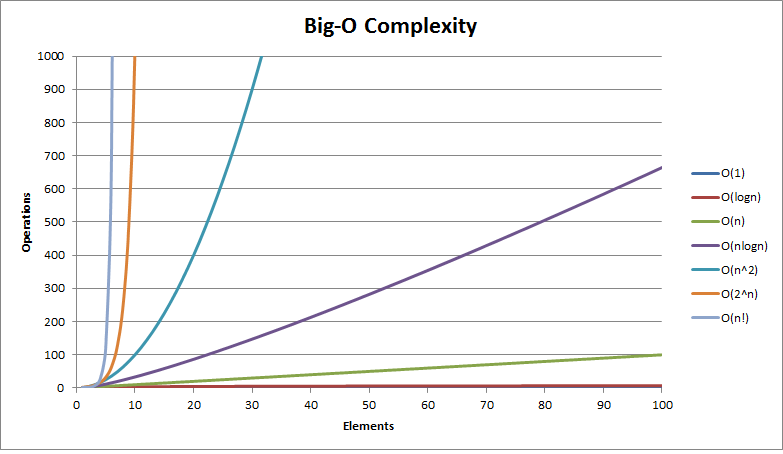
\includegraphics[width=0.9\textwidth]{images/big-o-complexity}
\end{center}

\end{frame}
\begin{frame}
  \frametitle{Parallelism versus Concurrency}

  Before we talk about parallelism, let's distinguish it from concurrency.

  {\bf Parallelism}

  Two or more tasks are \structure{parallel}\\ \hspace*{2em} if they are running at the same time. 

  Main goal: run tasks as fast as possible. 

  Main concern: \structure{dependencies}.
  \vfill
  {\bf Concurrency}

  Two or more tasks are \structure{concurrent}\\ \hspace*{2em} if the ordering of the two tasks is not 
  predetermined. 

  Main concern: \structure{synchronization}.

\end{frame}

\begin{frame}
  \frametitle{Limitations of Speedups}

    Our main focus is parallelization.\\[1em]
  \begin{itemize}
    \item Most programs have a sequential part and a parallel part; and,\\[1em]
    \item Amdahl's Law answers, ``what are the limits to parallelization?''
  \end{itemize}
  
  \begin{center}
	
\includegraphics[width=0.7\textwidth]{images/linedrawnhere.jpeg}
\end{center}

\end{frame}



\begin{frame}
\frametitle{Visualizing Amdahl's Law}

  \hspace*{2em}\begin{minipage}{.8\textwidth}
  $S$: fraction of serial runtime in a serial execution.

  $P$: fraction of parallel runtime in a serial execution.

  Therefore, $S + P = 1$.\\[2em]

  With 4 processors, best case, what can happen to the following runtime?
  \end{minipage}

  \hspace*{5em}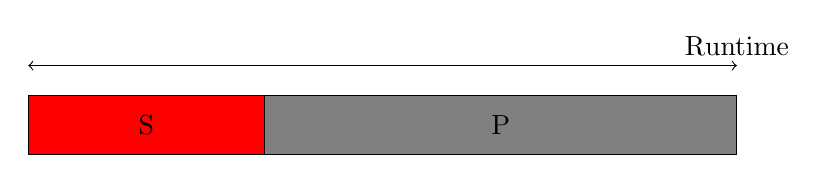
\begin{tikzpicture}
   \draw[<->] (-1.5,0.75) -- (7.5,0.75) node[above] {Runtime};
   \draw (0,0) node[rectangle, fill=red, minimum height=0.75cm, minimum width=3cm,draw] {S};
   \draw (4.5,0) node[rectangle, fill=gray, minimum height=0.75cm, minimum width=6cm,draw] {P};
  \end{tikzpicture}
\end{frame}

\begin{frame}
  \frametitle{Visualizing Amdahl's Law}

  \hspace*{5em}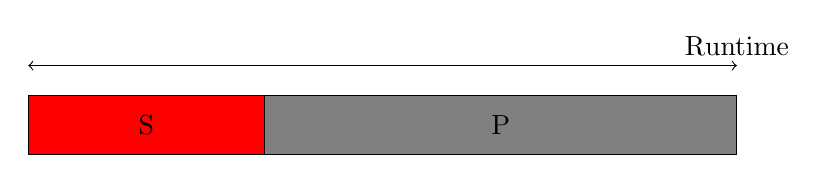
\begin{tikzpicture}
   \draw[<->] (-1.5,0.75) -- (7.5,0.75) node[above] {Runtime};
   \draw (0,0) node[rectangle, fill=red, minimum height=0.75cm, minimum width=3cm,draw] {S};
   \draw (4.5,0) node[rectangle, fill=gray, minimum height=0.75cm, minimum width=6cm,draw] {P};
  \end{tikzpicture}
  \vfill
  We want to split up the parallel part over 4 processors
  \vfill
  \hspace*{5em}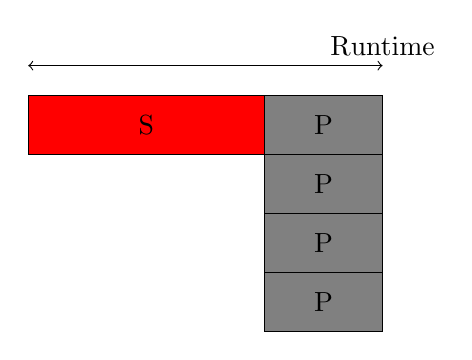
\begin{tikzpicture}
   \draw[<->] (-1.5,0.75) -- (3,0.75) node[above] {Runtime};
   \draw (0,0) node[rectangle, fill=red, minimum height=0.75cm, minimum width=3cm,draw] {S};
   \draw (2.25,0) node[rectangle, fill=gray, minimum height=0.75cm, minimum width=1.5cm,draw] {P};
   \draw (2.25,-0.75) node[rectangle, fill=gray, minimum height=0.75cm, minimum width=1.5cm,draw] {P};
   \draw (2.25,-1.5) node[rectangle, fill=gray, minimum height=0.75cm, minimum width=1.5cm,draw] {P};
   \draw (2.25,-2.25) node[rectangle, fill=gray, minimum height=0.75cm, minimum width=1.5cm,draw] {P};
  \end{tikzpicture}
\end{frame}

\begin{frame}
  \frametitle{Obey the Law}

\Large
$T_s$: time for the program to run in serial

$N$: number of processors/parallel executions

$T_p$: time for the program to run in parallel
\vfill
  \begin{itemize}
    \item Under perfect conditions, get $N$ speedup for $P$
  \end{itemize}
\vfill

  \begin{center}
$T_p = T_s \cdot (S + \frac{P}{N})$
  \end{center}
\end{frame}

\begin{frame}
  \frametitle{Obey the Law}

  \hspace*{3em} How much faster can we make the program?

  \begin{eqnarray*}
  \mbox{\em speedup} &=& \frac{T_s}{T_p}\\
                     &=& \frac{T_s}{T_S \cdot (S + \frac{P}{N})}\\
                     &=& \frac{1}{S + \frac{P}{N}}
  \end{eqnarray*}
  \vfill
  \hspace*{3em} (assuming no overhead for parallelizing; or costs near
  zero)

\end{frame}

\begin{frame}
  \frametitle{Fixed-Size Problem Scaling, \\ Varying Fraction of Parallel Code}

  \begin{center}
    \hspace*{2em}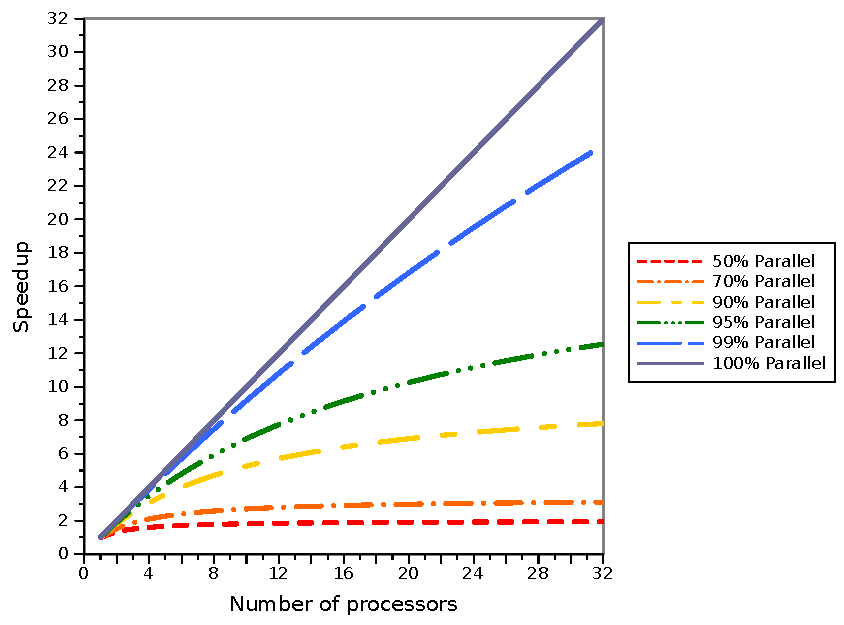
\includegraphics[scale=0.68]{images/parallel-scaling.pdf}
  \end{center}
\end{frame}


\begin{frame}
  \frametitle{Amdahl's Law}

 \hspace*{2em}Replace $S$ with $(1 - P)$:

  \begin{center}
    \structure{$\mbox{\em speedup} = \frac{1}{(1 - P) + \frac{P}{N}}$}
  \end{center}
  \vfill
  \begin{center}
    $\mbox{\em maximum speedup} = \frac{1}{(1 - P)}$, since $\frac{P}{N} \rightarrow 0$
  \end{center}

As you might imagine, the asymptotes in the previous graph are bounded by the
  maximum speedup.
\end{frame}

\begin{frame}
\frametitle{Speedup Example}


Suppose: a task that can be executed in 5~s, containing a parallelizable loop.

Initialization and recombination code in this routine requires 400~ms. 

So with one processor executing, it would take about 4.6~s to execute the loop. 

Split it up and execute on two processors: about 2.3~s to execute the loop. 

Add to that the setup and cleanup time of 0.4~s and we get a total time of 2.7~s. 

Completing the task in 2.7~s rather than 5~s represents a speedup of about~46\%.

\end{frame}


\begin{frame}
\frametitle{Amdahl's Law on the 5~s Task}

Applying this formula to the example:

\begin{center}
	\begin{tabular}{l|l}
	\textbf{Processors} & \textbf{Run Time (s)} \\ \hline
	1 & 5\\
	2 & 2.7\\
	4 & 1.55\\
	8 & 0.975\\
	16 & 0.6875 \\
	32 & 0.54375 \\
	64 & 0.471875 \\
	128 & 0.4359375\\
	\end{tabular}
\end{center}

\end{frame}

 
\begin{frame}
\frametitle{Observations on the 5~s Task}

1. Diminishing returns as we add more processors.

2. Converges on 0.4~s.

The most we could speed up this code is by a factor of $\frac{5}{0.4}\approx 12.5$.

But that would require infinite processors (and therefore infinite money).

\end{frame}

\begin{frame}
  \frametitle{Assumptions behind Amdahl's Law}

    We assume:
    \begin{itemize}
    \item problem size is fixed (we'll see this soon);
    \item program/algorithm behaves the same on 1 processor and on $N$ processors;
    \item that we can accurately measure runtimes---\\ ~~i.e. that overheads don't matter.
    \end{itemize}
    
    \begin{center}
	
\includegraphics[width=0.6\textwidth]{images/overhead.jpg}
	\end{center}
  
\end{frame}

\begin{frame}
  \frametitle{Amdahl's Law Generalization}

  \hspace*{2em} The program may have many parts, each of which we can tune to
  a different degree.\\[1em]

  Let's generalize Amdahl's Law.\\[1em]

  $f_1, f_2, \ldots, f_n$: fraction of time in part $n$

  $S_{f_1}, S_{f_n}, \ldots, S_{f_n}$: speedup for part $n$

  \vfill
  \begin{center}
  \structure{\[\mbox{\em speedup} = \frac{1}{\frac{f_1}{S_{f_1}} + \frac{f_2}{S_{f_2}} + \ldots +
    \frac{f_n}{S_{f_n}}}\]}
  \end{center}
\end{frame}


\begin{frame}
  \frametitle{Application (1)}

  \hspace*{2em} 
Consider a program with 4 parts in the following scenario:\\[2em]
    \begin{tabular}{r|r|r|r}
    \multicolumn{2}{l}{} & \multicolumn{2}{c}{Speedup} \\
    Part & Fraction of Runtime & Option 1 & Option 2\\
    \hline
    1 & 0.55 & 1  & 2\\
    2 & 0.25 & 5  & 1\\
    3 & 0.15 & 3  & 1\\
    4 & 0.05  & 10 & 1\\
  \end{tabular}

~\\[2em]
  We can implement either Option 1 or Option 2. \\
  Which option is better?

\end{frame}

\begin{frame}
  \frametitle{Application (2)}


  \hspace*{2em} ``Plug and chug'' the numbers:\\[1em]

  {\bf Option 1} \vspace*{-2em}

  \[ \mbox{\em speedup} = \frac{1}{0.55 + \frac{0.25}{5} + \frac{0.15}{3} + \frac{0.05}{5}}
    = 1.53  \]
~\\[1em]
  {\bf Option 2} \vspace*{-2em}

   \[\mbox{\em speedup} = \frac{1}{\frac{0.55}{2} + 0.45} = 1.38 \hspace*{5.5em}\]


\end{frame}

\begin{frame}
  \frametitle{Empirically estimating parallel speedup P}

  \hspace*{2em} Useful to know, don't have to commit to memory:
  \vfill
  \[P_{\mbox{\scriptsize estimated}} = \frac{\frac{1}{\mbox{\em speedup}}-1}{\frac{1}{N}-1}\]
  \vfill
  \hspace*{2em} \begin{minipage}{.8\textwidth} \begin{itemize}
    \item Quick way to guess the fraction of parallel code
    \item Use $P_{\mbox{\scriptsize estimated}}$ to predict speedup for a different number of processors
  \end{itemize} \end{minipage}
\end{frame}

\begin{frame}
  \frametitle{Summary of Amdahl's Law}

\hspace*{2em} Important to focus on the part of the program with most impact.\\[1em]

\hspace*{2em} Amdahl's Law:\\[1em]
\hspace*{2em}
  \begin{itemize}
    \item estimates perfect performance gains from
          parallelization (under assumptions); but,
    \vfill
    \item only applies to solving a \structure{fixed problem size} in the
          shortest possible period of time
  \end{itemize}
\end{frame}

\begin{frame}
  \frametitle{Gustafson's Law: Formulation}

\hspace*{2em} 
\begin{tabbing}
  $n$:~~~~~~ \= problem size\\[.1em]

  $S(n)$: \> fraction of serial runtime for a parallel execution\\[.1em]

  $P(n)$: \> fraction of parallel runtime for a parallel execution\\
\end{tabbing}


\begin{eqnarray*}
T_p &=& S(n) + P(n) = 1 \\
T_s &=& S(n) + N \cdot P(n) 
\end{eqnarray*}

\[ \mbox{\em speedup} = \frac{T_s}{T_p} \]
\end{frame}

\begin{frame}
  \frametitle{Gustafson's Law}

\hspace*{2em}
  \structure{$speedup = S(n) + N \cdot P(n)$}\\[1em]

  Assuming the fraction of runtime in serial part decreases as $n$ increases,
  the speedup approaches $N$.


Yes! Large problems can be efficiently parallelized. (Ask Google.)

\end{frame}

\begin{frame}
  \frametitle{Driving Metaphor}

  {\bf Amdahl's Law}
  
  Suppose you're travelling between 2 cities 90~km apart. If you travel for an
  hour at a constant speed less than 90 km/h, your average will never equal
  90~km/h, even if you energize after that hour.
  \vfill
  {\bf Gustafson's Law}

  Suppose you've been travelling at a constant speed less than 90~km/h. Given
  enough distance, you can bring your average up to 90~km/h.
\end{frame}

\part{Parallelization Techniques}
\begin{frame}
\partpage
\begin{center}
	
\includegraphics[width=0.25\textwidth]{images/cutup.jpg}
\end{center}
\end{frame}

\begin{frame}
\frametitle{Lock It Down}
The more locks and locking we need, the less scalable the code is going to be. 

You may think of the lock as a resource. 
The more threads or processes that are looking to acquire that lock, the more ``resource contention'' we have.

And thus more waiting and coordination are going to be necessary.

\end{frame}

\begin{frame}
\frametitle{``We have a new enemy...''}

Assuming we're not working with an embedded system where all memory is statically allocated in advance, there will be dynamic memory allocation. 

The memory allocator is often centralized and may support only one thread allocating or deallocating at a time (using locks to ensure this). 

This means it does not necessarily scale very well.

There are some techniques for dynamic memory allocation that allow these things to work in parallel.


\end{frame}


\begin{frame}
\frametitle{Everybody Into the Pool}

If we have a pool of workers, the application just submits units of work, and then on the other side these units of work are allocated to workers. 

The number of workers will scale based on the available hardware. 

This is neat as a programming practice: as the application developer we don't care quite so much about the underlying hardware. 

Let the operating system decide how many workers there should be, to figure out the optimal way to process the units of work.

\end{frame}


\begin{frame}[fragile]
\frametitle{Rust Thread Pool}

\begin{lstlisting}[language=Rust]
use std::collections::VecDeque;
use std::sync::{Arc, Mutex};
use threadpool::ThreadPool;
use std::thread;

fn main() {
    let pool = ThreadPool::new(8);
    let queue = Arc::new(Mutex::new(VecDeque::new()));
    println!("main thread has id {}", thread_id::get());

    for j in 0 .. 4000 {
        queue.lock().unwrap().push_back(j);
    }
    queue.lock().unwrap().push_back(-1);
\end{lstlisting}


\end{frame}
\begin{frame}[fragile]
\frametitle{Rust Thread Pool}

\begin{lstlisting}[language=Rust]
    for i in 0 .. 4 {
        let queue_in_thread = queue.clone();
        pool.execute(move || {
            loop {
                let mut q = queue_in_thread.lock().unwrap();
                if !q.is_empty() {
                    let val = q.pop_front().unwrap();
                    if val == -1 {
                        q.push_back(-1);
                        println!("Thread {} got the signal to exit.", thread_id::get());
                        return;
                    }
                    println!("Thread {} got: {}!", thread_id::get(), val);
                }
            }
        });
    }
    pool.join();
}
\end{lstlisting}


\end{frame}


\begin{frame}[fragile]
\frametitle{Thread Pool Output}


\begin{verbatim}
main thread has id 4455538112
Thread 123145474433024 got: 0!
Thread 123145474433024 got: 1!
Thread 123145474433024 got: 2!

...

Thread 123145478651904 got: 3997!
Thread 123145478651904 got: 3998!
Thread 123145478651904 got: 3999!
Thread 123145476542464 got the signal to exit.
Thread 123145484980224 got the signal to exit.
Thread 123145474433024 got the signal to exit.
Thread 123145478651904 got the signal to exit.
\end{verbatim}


\end{frame}




\part{Threads vs Processes}
\begin{frame}
\partpage
\begin{center}
	
\includegraphics[width=0.5\textwidth]{images/marvelvsdc.jpg}
\end{center}
\end{frame}


\begin{frame}[fragile]
  \frametitle{Background}


  Recall the difference between \structure{processes} and 
          \structure{threads}:
  \begin{itemize}
    \item Threads are basically light-weight processes which piggy-back on
          processes' address space.
  \end{itemize} ~\\
  Traditionally (pre-Linux 2.6) you had to use {\tt fork}~(for~processes) and {\tt clone} (for threads).


\end{frame}

\begin{frame}[fragile]
  \frametitle{History}


    Developers mostly used {\tt fork} before there was a standardized way to create threads ({\tt clone} was non-standards-compliant).

  For performance reasons, along with ease and consistency, we'll use
  \structure{Pthreads}.

  {\tt fork} creates a new process.
      \begin{itemize}
        \item Drawbacks?
        \item Benefits?
      \end{itemize}
  
\end{frame}

\begin{frame}[fragile]
  \frametitle{Benefit: {\tt fork} is Safer and More Secure Than Threads}

  \begin{enumerate}
    \item Each process has its own virtual address space:
      \begin{itemize}
        \item Memory pages are not copied, they are copy-on-write---
        \item Therefore, uses less memory than you would expect.
      \end{itemize}
    \item Buffer overruns or other security holes do not expose other~processes.
    \item If a process crashes, the others can continue.
  \end{enumerate}~\\[1em]
  {\bf Example:} In the Chrome browser, each tab is a separate process.
\end{frame}

\begin{frame}[fragile]
  \frametitle{Drawback of Processes: Threads are Easier and Faster}

  \begin{itemize}
    \item Interprocess communication (IPC) is more complicated and slower than interthread
          communication.
      \begin{itemize}
        \item Need to use operating system utilities (pipes, semaphores, shared
              memory, etc) instead of thread library (or just memory reads and writes).
      \end{itemize}
    \item Processes have much higher startup, shutdown and synchronization cost.
    \item And, \structure{Pthreads}/\structure{C++11 threads} fix issues\\ with {\tt clone} and provide a
          uniform interface for most systems {\bf (Assignment 1)}.
  \end{itemize}

\end{frame}

\begin{frame}[fragile]
  \frametitle{Appropriate Time to Use Processes}


  If your application is like this:
  \begin{itemize}
    \item Mostly independent tasks, with little or no communication.
    \item Task startup and shutdown costs are negligible compared to overall runtime.
    \item Want to be safer against bugs and security holes.
  \end{itemize}
  Then processes are the way to go. \\[1em]


\end{frame}

\begin{frame}[fragile]
\frametitle{Threads vs Processes: Rust}

\begin{multicols}{2}

\begin{lstlisting}[language=Rust]
use std::process::Command;

fn main() {
    for j in 0 .. 50000 {
       Command::new("/bin/false").spawn();
    }
}
\end{lstlisting}
\begin{verbatim}
1.530 s +/-  0.134 s
\end{verbatim}
\columnbreak
\begin{lstlisting}[language=Rust]
use std::thread;

fn main() {
    for j in 0 .. 50000 {
        thread::spawn(|| {
            false
        });
    }
}
\end{lstlisting}
\begin{verbatim}
630.5 ms +/-  21.5 ms 
\end{verbatim}

\end{multicols}

  
\end{frame}

%%%%%%%%%%%%%%%%%%%%%%%%%%%%%%%%%%%%%%%%%%%%%%%%%%%%%%%%%%%%%%%%%%%%%%%%%%%%%%%%
\begin{frame}
  \frametitle{Task-Based Patterns: Overview}

  
  \begin{itemize}
    \item We'll now look at thread and process-based~parallelization.
    \item Although threads and processes differ, we don't care for now.
  \end{itemize}
  
  \begin{center}
	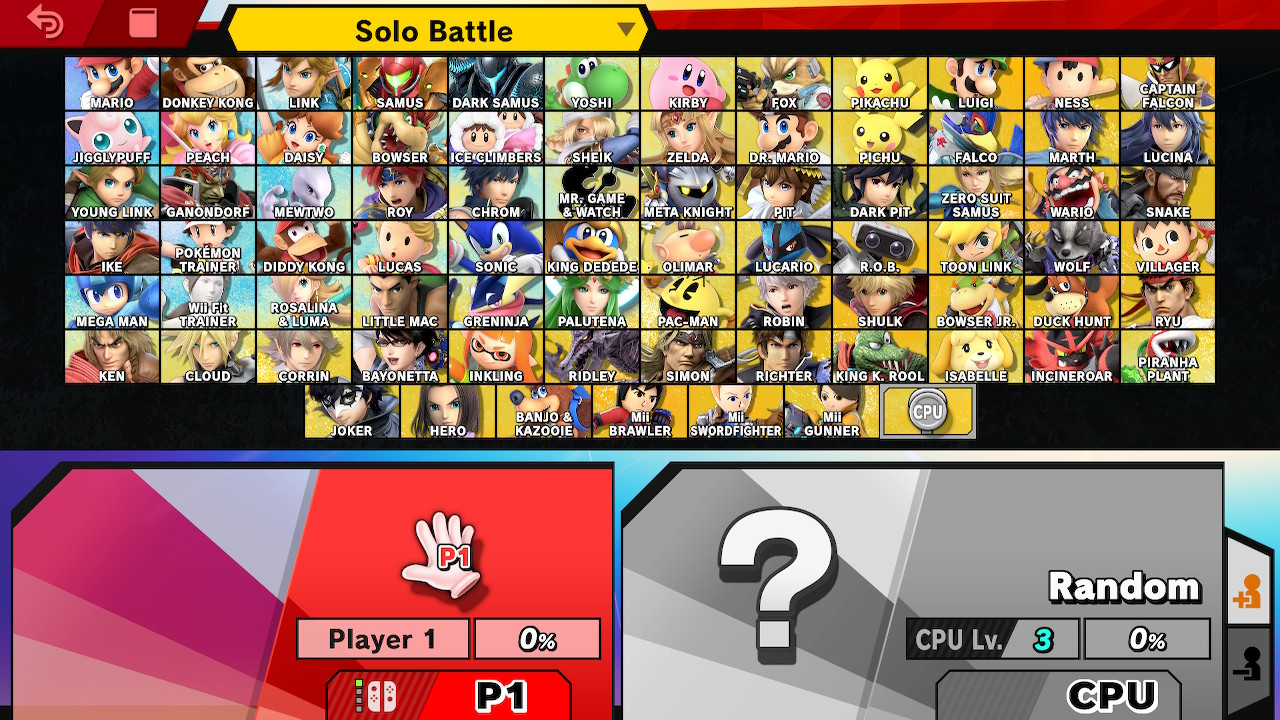
\includegraphics[width=\textwidth]{images/characterselect.jpeg}
  \end{center}

\end{frame}
%%%%%%%%%%%%%%%%%%%%%%%%%%%%%%%%%%%%%%%%%%%%%%%%%%%%%%%%%%%%%%%%%%%%%%%%%%%%%%%%

%%%%%%%%%%%%%%%%%%%%%%%%%%%%%%%%%%%%%%%%%%%%%%%%%%%%%%%%%%%%%%%%%%%%%%%%%%%%%%%%
\begin{frame}
  \frametitle{Pattern 1: Multiple Independent Tasks}

  
    Only useful to maximize system utilization.
  \begin{itemize}
    \item Run multiple tasks on the same system \\ ~~~(e.g. database and web server).\\[1em]
     If one is memory-bound and the other is I/O-bound, for example, you'll
      get maximum utilization out of your resources.\\[1em]
     {\bf Example:} cloud computing, each task is independent and can
      tasks can spread themselves over different nodes.\\[1em]
    \item Performance can increase linearly with the number of threads.
  \end{itemize}
  
\end{frame}
%%%%%%%%%%%%%%%%%%%%%%%%%%%%%%%%%%%%%%%%%%%%%%%%%%%%%%%%%%%%%%%%%%%%%%%%%%%%%%%%

%%%%%%%%%%%%%%%%%%%%%%%%%%%%%%%%%%%%%%%%%%%%%%%%%%%%%%%%%%%%%%%%%%%%%%%%%%%%%%%%
\begin{frame}
  \frametitle{Pattern 2: Multiple Loosely-Coupled Tasks}

  
    Tasks aren't quite independent, so there needs to be some inter-task
      communication (but not much).
  \begin{itemize}

    \item Communication might be from the tasks to a controller or status
      monitor.
  \end{itemize}

    Refactoring an application can help with latency. \\
For instance: split off
      the CPU-intensive computations into a separate thread---your application may
      respond more quickly.\\[1em]
     {\bf Example:} A program (1) receives/forwards packets and (2) logs them. You
      can split these two tasks into two threads, so you can still
      receive/forward while waiting for disk. This will increase the
      \structure{throughput} of the system.
  
\end{frame}
%%%%%%%%%%%%%%%%%%%%%%%%%%%%%%%%%%%%%%%%%%%%%%%%%%%%%%%%%%%%%%%%%%%%%%%%%%%%%%%%

%%%%%%%%%%%%%%%%%%%%%%%%%%%%%%%%%%%%%%%%%%%%%%%%%%%%%%%%%%%%%%%%%%%%%%%%%%%%%%%%
\begin{frame}
  \frametitle{Pattern 3: Multiple Copies of the Same Task}

  
    Variant of multiple independent tasks: run multiple copies of the same task (probably on different data).

  \begin{itemize}
    \item No communcation between different copies.
  \end{itemize}

  Again, performance should increase linearly with number of tasks.\\[1em]

  {\bf Example:} In a rendering application, each thread can be
      responsible for a frame (gain \structure{throughput}; same
      \structure{latency}).

  
\end{frame}
%%%%%%%%%%%%%%%%%%%%%%%%%%%%%%%%%%%%%%%%%%%%%%%%%%%%%%%%%%%%%%%%%%%%%%%%%%%%%%%%

%%%%%%%%%%%%%%%%%%%%%%%%%%%%%%%%%%%%%%%%%%%%%%%%%%%%%%%%%%%%%%%%%%%%%%%%%%%%%%%%
\begin{frame}
  \frametitle{Pattern 4: Single Task, Multiple Threads}

  
  Classic vision of ``parallelization''.\\[1em]

  {\bf Example:} Distribute array processing over multiple 
      threads---each thread computes results for a subset of the array.

  \begin{itemize}
    \item Can decrease \structure{latency} (and increase
      \structure{throughput}), as we saw with \structure{Amdahl's Law}.
    \item Communication can be a problem, if the data is not nicely partitioned.
    \item Most common implementation is just creating threads and joining them,
      combining all results at the join.
  \end{itemize}
  
\end{frame}
%%%%%%%%%%%%%%%%%%%%%%%%%%%%%%%%%%%%%%%%%%%%%%%%%%%%%%%%%%%%%%%%%%%%%%%%%%%%%%%%

%%%%%%%%%%%%%%%%%%%%%%%%%%%%%%%%%%%%%%%%%%%%%%%%%%%%%%%%%%%%%%%%%%%%%%%%%%%%%%%%
\begin{frame}
  \frametitle{Pattern 5: Pipeline of Tasks}

  
    Seen briefly in computer architecture.

    \begin{itemize}
    \item Use multiple stages; each thread handles a stage.\\[1em]
     {\bf Example:} a program that handles network packets: (1) accepts
      packets, (2) processes them, and (3) re-transmits them. Could set up the threads such that each packet goes through the threads.
    \vfill
    \item Improves \structure{throughput}; may increase \structure{latency} as
      there's communication between threads.
    \vfill
    \item In the best case, you'll have a linear speedup.\\[1em]

     Rare, since the runtime of the stages will vary, and the slow
      one will be the bottleneck (but you could have 2 instances of the
      slow stage).
  \end{itemize}
  
\end{frame}
%%%%%%%%%%%%%%%%%%%%%%%%%%%%%%%%%%%%%%%%%%%%%%%%%%%%%%%%%%%%%%%%%%%%%%%%%%%%%%%%

%%%%%%%%%%%%%%%%%%%%%%%%%%%%%%%%%%%%%%%%%%%%%%%%%%%%%%%%%%%%%%%%%%%%%%%%%%%%%%%%
\begin{frame}
  \frametitle{Pattern 6: Client-Server}

  
    To execute a large computation, the server supplies work to many
      clients---as many as request it.\\[1em]

    Client computes results and returns them to the server.\\[1em]
   {\bf Examples:} botnets, {\tt SETI@Home}, GUI application (backend
      acts as the server).\\[1em]
   Server can arbitrate access to shared resources (such as network
      access) by storing the requests and sending them out.\\[1em]

   \begin{itemize}
    \item Parallelism is somewhere between single task, multiple threads and
      multiple loosely-coupled tasks  
  \end{itemize}
  
\end{frame}
%%%%%%%%%%%%%%%%%%%%%%%%%%%%%%%%%%%%%%%%%%%%%%%%%%%%%%%%%%%%%%%%%%%%%%%%%%%%%%%%

%%%%%%%%%%%%%%%%%%%%%%%%%%%%%%%%%%%%%%%%%%%%%%%%%%%%%%%%%%%%%%%%%%%%%%%%%%%%%%%%
\begin{frame}
  \frametitle{Pattern 7: Producer-Consumer}

  
    Variant on the pipeline and client-server models.\\
    Producer generates work, and consumer performs work.\\[1em]
    {\bf Example:} producer which generates rendered frames;
      consumer which orders these frames and writes them to disk.\\[1em]
    Any number of producers and consumers.\\[1em]

    \begin{itemize}
    \item This approach can improve \structure{throughput} and also reduces
      design complexity
    \end{itemize}
  
\end{frame}
%%%%%%%%%%%%%%%%%%%%%%%%%%%%%%%%%%%%%%%%%%%%%%%%%%%%%%%%%%%%%%%%%%%%%%%%%%%%%%%%

%%%%%%%%%%%%%%%%%%%%%%%%%%%%%%%%%%%%%%%%%%%%%%%%%%%%%%%%%%%%%%%%%%%%%%%%%%%%%%%%
\begin{frame}
  \frametitle{Combining Strategies}

\begin{center}
	
\includegraphics[width=0.6\textwidth]{images/fusion.jpeg}
\end{center}
  
    Most problems don't fit into one category;  it's often best to combine
      strategies.

    For instance, you might often start with a pipeline, and then use
      multiple threads in a particular pipeline stage to handle one piece of
      data.

  

\end{frame}
%%%%%%%%%%%%%%%%%%%%%%%%%%%%%%%%%%%%%%%%%%%%%%%%%%%%%%%%%%%%%%%%%%%%%%%%%%%%%%%%

%%%%%%%%%%%%%%%%%%%%%%%%%%%%%%%%%%%%%%%%%%%%%%%%%%%%%%%%%%%%%%%%%%%%%%%%%%%%%%%%
\begin{frame}
  \frametitle{Midterm Questions from 2011 (1)}


  For each of the following situations, {\bf name an appropriate parallelization
  pattern and the granularity at which you would apply it, explain the necessary
  communication, and explain why your pattern is appropriate}.
  \begin{itemize}
  \item build system, e.g. parallel make
    \begin{itemize}
      \item<2-> Multiple independent tasks, at a per-file granularity
    \end{itemize}
  \item optical character recognition system
    \begin{itemize}
      \item<2-> Pipeline of tasks
      \item<2-> 2 tasks - finding characters and analyzing them
    \end{itemize}
  \end{itemize}

\end{frame}
%%%%%%%%%%%%%%%%%%%%%%%%%%%%%%%%%%%%%%%%%%%%%%%%%%%%%%%%%%%%%%%%%%%%%%%%%%%%%%%%

%%%%%%%%%%%%%%%%%%%%%%%%%%%%%%%%%%%%%%%%%%%%%%%%%%%%%%%%%%%%%%%%%%%%%%%%%%%%%%%%
\begin{frame}
  \frametitle{Midterm Questions from 2011 (2)}


  {\bf Give a concrete example} where you would use the following
  parallelization patterns. {\bf Explain} the granularity at which you'd apply
  the pattern.
  \begin{itemize}
    \item single task, multiple threads:
    \begin{itemize}
      \item<2-> Computation of a mathematical function with independent
        sub-formulas.
    \end{itemize}
    \item producer-consumer (no rendering frames, please):
    \begin{itemize}
      \item<2-> Processing of stock-market data:
        a server might generate raw financial data (quotes) for a
        particular security. The server would be the producer. Several clients
        (or consumers) may take the raw data and use them in different ways, e.g. by computing means, generating charts, etc.
    \end{itemize}
  \end{itemize}
 
\end{frame}
%%%%%%%%%%%%%%%%%%%%%%%%%%%%%%%%%%%%%%%%%%%%%%%%%%%%%%%%%%%%%%%%%%%%%%%%%%%%%%%%

\end{document}

